\section{Implementation}
In the following we want to describe implementation specific details of both the simulator as well as the map editing application. We will elucidate problems we faced during the implementation and the integration of both applications and how we solved them. 
\subsection{Simulator}
Behind the user interface of the simulator a continuously running thread is mandated with updating the current state of the simulation with each tick, i.e. every 50ms. The thread execution is triggered by the globally governing SimulationController and its \textit{run}-method (fig. \ref{sd_animthread}) appears refreshingly simple. Despite the apparent simplicity the design of the thread posed a range of problems. As is usual for Java UI frameworks, JavaFX also prohibits changes to UI objects by any thread other the main application thread, forcing us to submit each update that is to be escalated to the interface as a \textit{runnable} object to said application thread's execution queue. To reduce scheduling overhead we kept the AnimationThread's main loop as simple as possible, resulting in no more than four calls to the mentioned execution queue. 

\begin{figure}[h]
	\begin{center}
		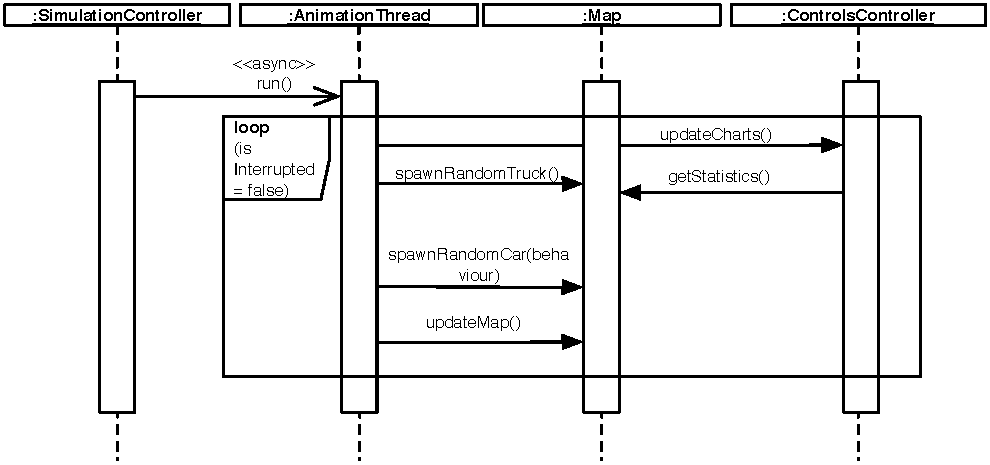
\includegraphics[width=\textwidth]{img/SD_animThread.pdf}
		\caption[Sequence Diagram of the Animation Thread]{Sequence Diagram of the Animation Thread}
		\label{sd_animthread}
	\end{center}
\end{figure}

With the multithreaded execution described above came concurrency related issues. The class Map contains a list to all vehicles currently present in the simulation. Whenever a vehicle is leaving the map, it notifies the SimulationController, which in turn removes the vehicle from the simulation. As the map's \textit{updateMap()} is constantly iterating through its list of vehicles, removing a vehicle from anywhere else than within this loop results in concurrency exceptions.

\begin{wrapfigure}{r}{0.45\textwidth}
	\begin{minipage}{0.45\textwidth}
		\begin{lstlisting}[caption={Car Removal}, label={lst_carRem}]
if(toBeRemoved.contains(v)){
	iter.remove();
	toBeRemoved.remove(v);
	continue;
}	
		\end{lstlisting}
	\end{minipage}
\end{wrapfigure}

In order to overcome this issue we considered both the traditional reader-writer-locking as well as the more advanced read-copy-update pattern, but eventually come to the conclusion but using either of them will introduce an additional scheduling (and implementation) overhead and hence only yield imperceptible performance improvements over the solution we employed (listing \ref{lst_carRem}). As mentioned earlier, the \textit{updateMap()} method loops through all existing vehicles with each tick, we create a list of vehicles that are about to move the map within the next tick. As soon as the iterator (\textit{iter}) points to a vehicle \textit{v} that is on the \textit{toBeRemoved} list, it is removed and the loop skips one iteration.  

In order to ease the communication between model classes and the \textit{SimulationController} as well as the application classes \textit{MainApp} and \textit{EditorApp} we faced a design decision between the traditional observer pattern and the singleton pattern that allows static access to the required instances. We decided in favour of the singleton pattern, because the situations in which the model communicates with the \textit{SimulationController} are manifold and access to the singleton instance allows for fairly simple communication flows.

%TODO Testing: Jerry?
